\documentclass{article}

\usepackage{amsmath}
\usepackage{graphicx}
\usepackage{wrapfig}
\usepackage{listings}
\lstset{
basicstyle=\small\ttfamily,
columns=flexible,
breaklines=true
}
\usepackage{biblatex}
\usepackage{units}
\usepackage{xcolor}
\usepackage{float}
\definecolor{codegray}{rgb}{209,209,209}

\lstset{
    backgroundcolor=\color{codegray},
}

\newcommand{\qMain}{What is the relationship between normalized harmonic complexity and perceived enjoyment of the I - V - IV - iv chord progression?}

\newcommand{\qI}{How does the average normalized harmonic complexity of the I - V - IV - iv chord progression compare to different chord progressions?}

\newcommand{\qII}{How does the perceived enjoyment of the I - V - IV - iv chord progression compare to different chord progressions within audiences exposed to American music?} 

\newcommand{\rChord}{I - V - IV -iv}

\title{\qMain}
\author{Jonathan Elkouby}
\begin{document}
    \maketitle
    \begin{figure}
    
    \end{figure}
    \newpage
    \tableofcontents
    \section{Theoretical framework}
This research paper uses certain terms with ambiguous definitions. This section aims to explicitly state a definition of these terms.

\subsection{Partials, frequency ratios, triads, and harmonic complexity}

Over the course of this research paper, the ``\textbf{frequency of a note}'' is mentioned frequently. A necessary abstraction: this refers exclusively to the fundamental frequency of a note. Nuances to frequency (e.g. overtones) are treated as outside of the scope of this research. Also note that one or , or as a sine wave

\begin{figure}
% figure of a C4 on sheet
% figure of a C4 as a wave
\end{figure}

A frequency ratio is a relation between two or more partial frequencies. An interval is a relation of two notes, while a triad is a relation of three notes. Over the course of this research paper, a frequency ratio is expressed as two or more notes on sheet music, and their corresponding distance on the musical scale (e.g. a "major third" or "perfect fifth"), or as a mathematical ratio of the form $a : b$ (for intervals) or $a : b : c$ (for triads), where $a$, $b$, and $c$ are partial frequencies, respective in size. 

\ref{The Arithmetic of Listening}

% when said "progressions A to C", it is implied to be inclusive, meaning it includes \{A, B, C\}

% normalized harmonic complexity definition
% Reference the list of chord progressions A through J that is used throughout the course of the research paper
    \newpage
    \section{\qI}

\subsection{Introduction}
This subquestion is answered by calculating the normalized harmonic complexity of chord progressions A through J, then comparing chord progression C to the other chord progressions.

\subsection{Results}
The following is the standard output of \lstinline[]|data/q1/results.py|:

\begin{lstlisting}
Normalized harmonic complexity of A (octave) =  0.0
Normalized harmonic complexity of B (I_V_IV_IV) =  35.57
Normalized harmonic complexity of C (I_V_IV_iv) =  44.46
Normalized harmonic complexity of D (I_V_iv_iv) =  53.35
Normalized harmonic complexity of E (I_v_iv_iv) =  62.25
Normalized harmonic complexity of F (i_v_iv_iv) =  71.14
Normalized harmonic complexity of G (adj) =  100.0
Normalized harmonic complexity of H (I_V_vi_IV) =  44.46
Normalized harmonic complexity of I (I_V_vi_iii_IV) =  49.8
Normalized harmonic complexity of J (vi_V_IV_V) =  44.46   
\end{lstlisting}

These values were entered in an Excel sheet to create the following graph (figure 1):

\begin{figure}[H]
    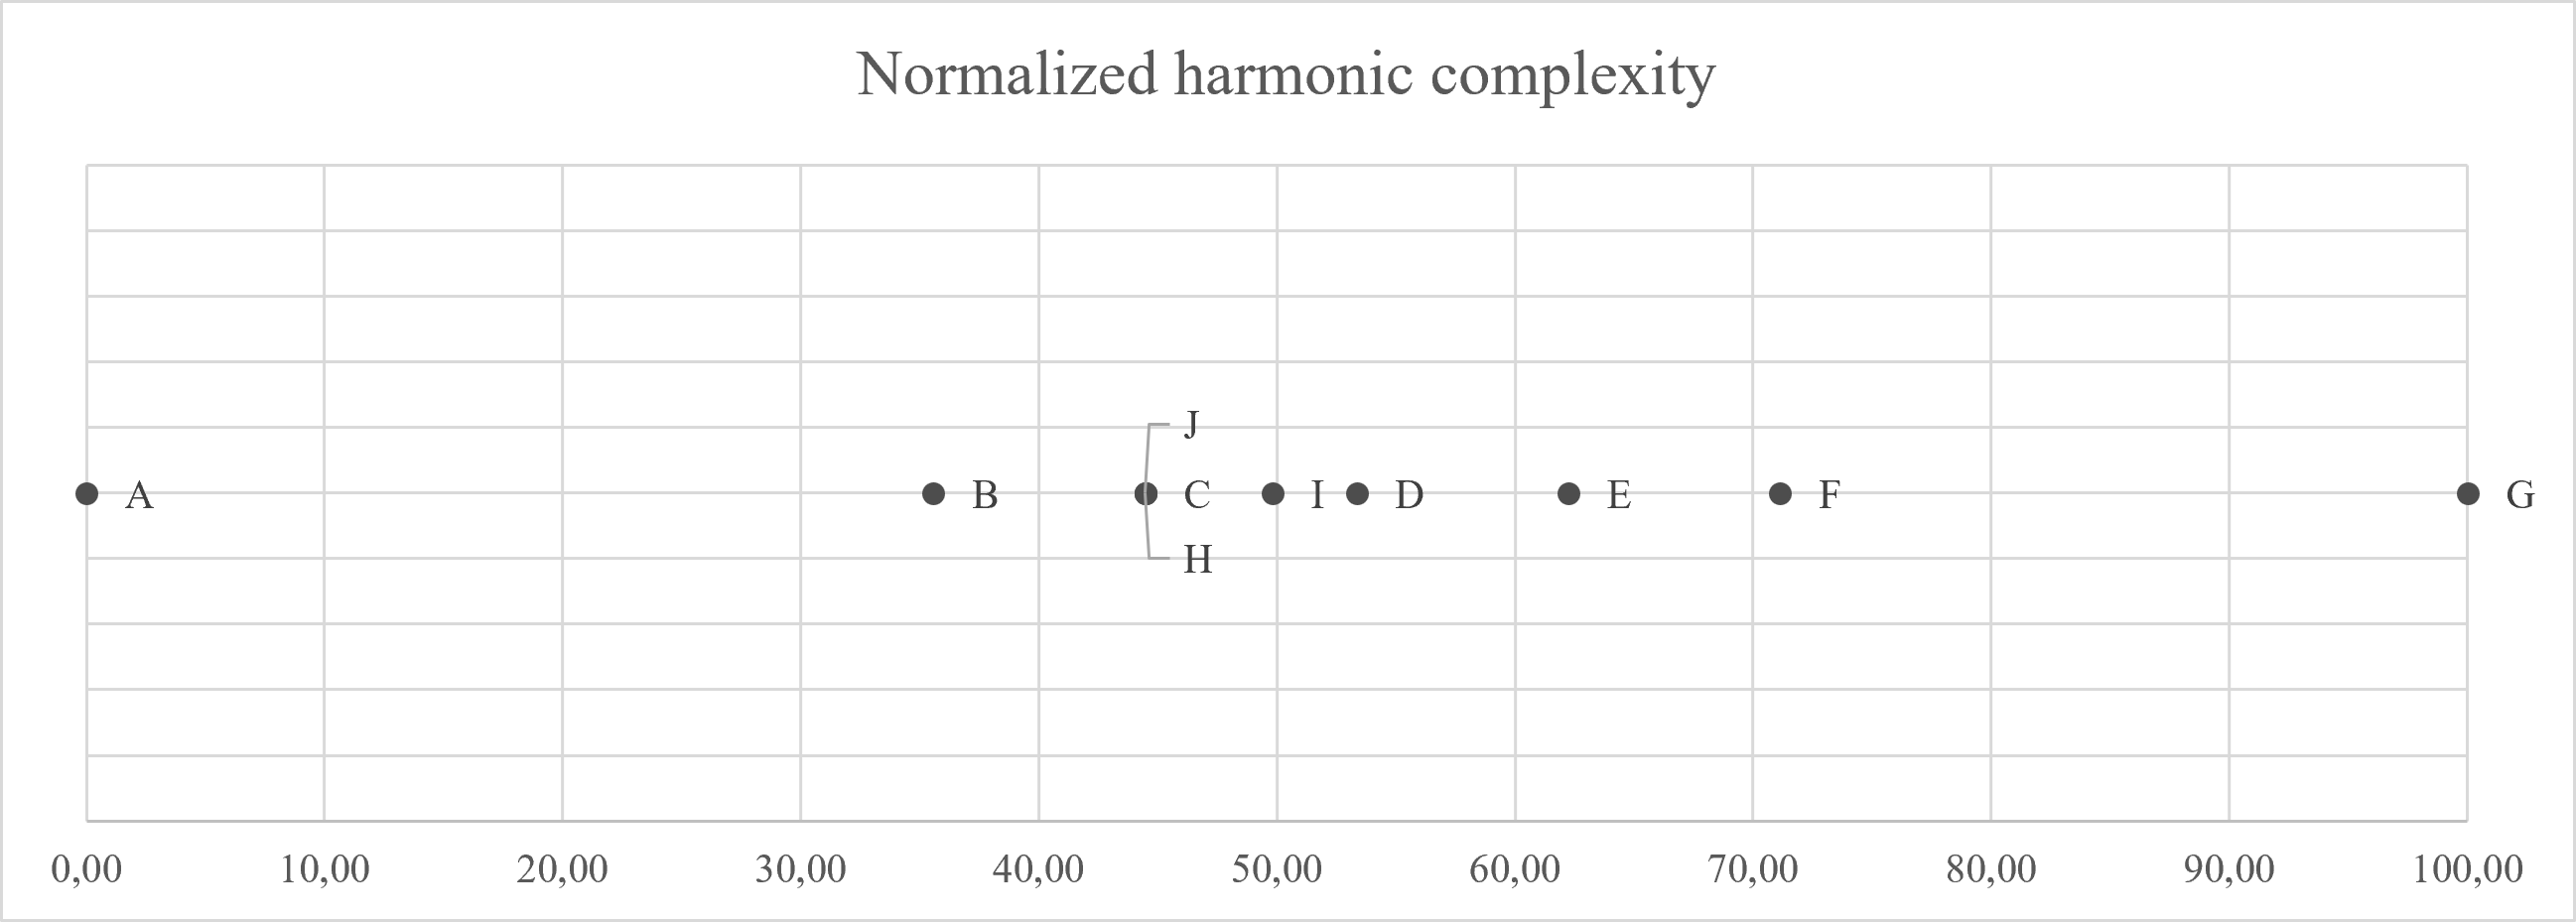
\includegraphics[width=\textwidth]{figures/q1/normalized_harmonic_complexity.png}
    \caption{Each dot resembles a chord progression. Its x-coordinate is equal to its harmonic complexity.}
\end{figure}


\subsection{Analysis \& Conclusion}
The calculations yield that chord progession C (I - V - IV - iv) has a normalized harmonic complexity of $44.46\% $, similar to chord progressions D and H through J.

We can also see that chord progressions A through F progressively increase in harmonic complexity, and that chord progression D is closest to a middle position (53\%) on a scale of 1 - 100\%. 
    \newpage
    \section{\qII}

\subsection{Introduction}
This subquestion can be answered by investigating empirical data of perceived enjoyment of a variety of chord progressions. The empirical data can be used then deciding the extent of perceived enjoyment upon initial, isolated observation.

\subsection{Results}
% RESULTS ANALYZED FROM 18/09/2026

\subsection{Analysis (discrete)}
The boxplots show that fragments C and J share the highest distribution of ratings overall. Fragment J has a higher average of approximately $4$, while fragment C has a lower average of approximately $3$.

Fragment C shares the same mean with fragments B, D, E, F, H, and I.

\subsection{Analysis (continuous)}
The results yield an inverted-U shaped relation of the perceived enjoyment as harmonic complexity increases, with only one fragment deviating significantly. 

For fragments A to C, the average rated enjoyment increases, and fragment C reaches the highest distribution of ratings. However, the following fragment D has a more centered distribution than C, signifying the start of a decline. While the following fragment E has a lower distribution of ratings, fragment F moves back to a centered distribution of 3. Then, fragment G has the lowest distribution of ratings, with almost all values being 1.

Fragments H to J, having a similar harmonic complexity to fragment C, also have a similar average perceived enjoyment. The mean of fragments H and I are equal to that of fragment C, though their distributions are lower; fragment J has a higher mean, but equal distribution to that of fragment C.

\subsection{Conclusion (discrete)}
% The discrete conclusion draws a conclusion from results analyzed in this subquestion.

Given that the I - V - IV - iv chord progression has the highest distribution of ratings overall, we can infer that the I - V - IV - iv has a moderately high shared perceived enjoyment upon initial listen. 

It is not uniquely higher than all other chord progressions, though; the I - vi - IV - V chord progression has not only a congruent distribution of ratings, but a higher mean, from which we can infer an even higher shared perceived enjoyment. Also, many other chord progression had an approximately congruent mean as the I - V - IV - iv chord progression, despite its higher distribution.

\subsection{Conclusion (continuous)}
% The continuous conclusion draws a conclusion using data from subquestion 1 as well as this subquestion.

Given that there is an inverted U-shaped relation between the harmonic complexity of chord progressions and the perceived enjoyment, with I - V - IV - iv having the overall highest distribution and mean of perceived enjoyment, we can infer that the I - V - IV - iv sits at the vertex of this shape. In subquestion 1, we established that perceived enjoyment in terms of harmonic complexity has an inverted U-shape known as the Wundt Curve. These results not only strengthen that conclusion, but also suggest that the I - V - IV - iv has a value of harmonic complexity at the vertex 
\end{document}

% constant color for all graphs: rgb(209, 209, 209); HEX: #d1d1d1